%---------- Inleiding ---------------------------------------------------------

\section{Inleiding}%
\label{sec:inleiding}
De explosieve groei van data en de toenemende vraag naar naadloze integraties tussen applicaties hebben de rol van Application Programming Interfaces (API's) centraal geplaatst in de hedendaagse softwareontwikkeling. Een goed ontworpen en gedocumenteerde API is niet langer een luxe, maar essentieel voor succes in het digitale landschap. Dit is met name relevant voor BrightAnalytics, een bedrijf dat een geavanceerd data-visualisatieplatform aanbiedt voor financiële rapportering en business intelligence. De kwaliteit, consistentie en efficiëntie van de API's die BrightAnalytics ontwikkelt, zijn van cruciaal belang voor de functionaliteit van hun producten, de integratie met andere systemen en het snel kunnen ontwikkelen van nieuwe features.

\bigskip

Tijdens mijn stage bij BrightAnalytics ontwikkel ik "BrightEats", een applicatie waarmee werknemers hun lunch kunnen bestellen. Deze applicatie is afhankelijk van een robuuste en goed ontworpen backend API. De ontwikkeling van deze API biedt een uitgelezen kans om de principes van RESTful API design te implementeren en te evalueren binnen de specifieke context van BrightAnalytics.

\bigskip

Veel bedrijven ondervinden echter uitdagingen bij het waarborgen van consistente, kwalitatief hoogwaardige API's. Zonder duidelijke richtlijnen en gestandaardiseerde processen kunnen inconsistenties in API-ontwerp ontstaan, wat kan leiden tot suboptimale performance, integratieproblemen en problemen bij het onderhoud van de codebase. Om deze uitdagingen het hoofd te bieden, is het essentieel om best practices te definiëren en te implementeren die de kwaliteit, consistentie en efficiëntie van API-ontwikkeling kunnen verbeteren.

\bigskip

Deze bachelorproef beoogt een antwoord te formuleren op de volgende onderzoeksvraag:

\begin{center}
\textbf{Welke concrete best practices, gebaseerd op REST, HATEOAS en OpenAPI, kunnen gedefinieerd worden om de kwaliteit, consistentie en onderhoudbaarheid te verhogen van API's?}
\end{center}

\bigskip

Deze vraag zal beantwoord worden aan de hand van de volgende onderzoeksdoelstellingen:

\begin{enumerate}
\item \textbf{Inzicht verwerven in RESTful API design:} Een diepgaande analyse van de principes van RESTful API design, HATEOAS en OpenAPI specificatie, met als doel deze te vertalen naar concrete richtlijnen en best practices die toepasbaar zijn binnen de technologische context van BrightAnalytics.
\item \textbf{Ontwikkeling showcase API:} De backend API van de BrightEats applicatie zal ontwikkeld worden conform de gedefinieerde best practices, als showcase en proof-of-concept voor toekomstige API-ontwikkeling binnen het bedrijf.
\item \textbf{Formuleren van aanbevelingen:} Op basis van de bevindingen van de implementatie van de best practices in de BrightEats API, zullen concrete aanbevelingen geformuleerd worden voor het gebruik van deze aanpak in andere API's.
\end{enumerate}

\bigskip

Deze bachelorproef is relevant voor een breed scala aan bedrijven die streven naar het optimaliseren van hun API-ontwikkelingsproces. Door de principes van RESTful API design te omarmen en te vertalen naar concrete richtlijnen, kan BrightAnalytics de ontwikkeling van hoogwaardige, schaalbare en toekomstbestendige API's garanderen. De BrightEats API zal zo dienen als een concrete blauwdruk voor de ontwikkeling van toekomstgerichte API's binnen het bedrijf.

\section{Literatuurstudie}%
\label{sec:literatuurstudie}

We leven in een wereld die steeds digitaler wordt. Bedrijven gebruiken software voor allerlei taken, van boekhouding tot klantbeheer en marketing. De hoeveelheid data die deze software genereert, neemt exponentieel toe \autocite{Phiri2022}. Experts schatten dat er in 2025 wereldwijd meer dan 200 zettabytes aan data zal worden gegenereerd, een duizelingwekkende hoeveelheid informatie \autocite{Morgan2024}. Die data kan heel waardevol zijn als ze op de juiste manier wordt gebruikt om strategische beslissingen te nemen, processen te optimaliseren en nieuwe producten en diensten te ontwikkelen. Maar vaak is het een hele uitdaging om die data te ontsluiten en bruikbaar te maken. Softwareoplossingen werken vaak los van elkaar, waardoor het delen van data en het automatiseren van processen complex en tijdrovend is.

\bigskip

API's, of Application Programming Interfaces, bieden een oplossing voor dit probleem. Een API fungeert als een soort digitale brug tussen verschillende softwaretoepassingen, waardoor ze op een veilige en gestandaardiseerde manier data kunnen uitwisselen en met elkaar kunnen communiceren. Voor bedrijven die data-gedreven inzichten willen ontsluiten en efficiënte integraties tussen systemen willen realiseren, zijn API's onmisbaar. Zo'n tool is pas echt krachtig wanneer hij vlot kan samenwerken met andere bedrijfssystemen, zoals boekhoudpakketten, CRM-systemen of rapportagetools.

\bigskip

REST (Representational State Transfer) is een veelgebruikte architectuur om API's te ontwerpen en bouwen \autocite{Eddouibi2017}. Die populariteit heeft REST te danken aan zijn eenvoud, schaalbaarheid en compatibiliteit met de standaarden van het internet. Dankzij REST kunnen ontwikkelaars op een flexibele en efficiënte manier API's bouwen die vlot kunnen omgaan met de almaar toenemende hoeveelheid data die bedrijven vandaag genereren. In de volgende secties zullen we dieper ingaan op de principes en voordelen van RESTful API's.

\section{De principes van RESTful API's}

RESTful API's zijn gebaseerd op een aantal belangrijke principes die bijdragen aan hun eenvoud, schaalbaarheid en gebruiksvriendelijkheid. Eén van die principes is de client-server architectuur \autocite{Fielding2000}. Een RESTful API maakt een duidelijke scheiding tussen de client, die een aanvraag doet (bijvoorbeeld een rapport opvragen), en de server, die de aanvraag verwerkt en een antwoord terugstuurt. Deze scheiding zorgt ervoor dat de client en server onafhankelijk van elkaar kunnen evolueren, wat de flexibiliteit en onderhoudbaarheid ten goede komt.

\bigskip

Een ander belangrijk principe is statelessness, wat betekent dat elke request van de client naar de server alle informatie bevat die nodig is om de request te verwerken \autocite{Fielding2000}. De server hoeft dus geen informatie over de client bij te houden tussen verschillende requests. Dit maakt RESTful API's schaalbaarder, omdat servers requests parallel kunnen verwerken zonder afhankelijk te zijn van eerdere interacties. Bovendien wordt de betrouwbaarheid verhoogd, omdat een servercrash geen dataverlies veroorzaakt aan de clientzijde.

\bigskip

Cacheability is een derde belangrijk principe van REST  \autocite{Fielding2000}. Responses van de server kunnen gemarkeerd worden als cacheable, wat betekent dat de client (of een tussenliggende server) de response mag opslaan en hergebruiken voor latere, identieke requests. Caching vermindert de belasting van de server en verkort de laadtijden voor de gebruiker, wat de performantie van de applicatie ten goede komt.

\bigskip

Een uniform interface is een ander cruciaal aspect van RESTful API's. Dit betekent dat alle resources (bijvoorbeeld financiële rapporten, klanten, transacties) benaderd worden via eenzelfde set van operaties, gedefinieerd door de HTTP-methodes (GET, POST, PUT, DELETE) \autocite{Fielding2000}. Deze uniformiteit maakt de API voorspelbaar en gemakkelijk te gebruiken, omdat ontwikkelaars niet hoeven te leren hoe ze met elk type resource op een andere manier moeten omgaan.

\bigskip

Tot slot is het principe van een gelaagde systeemarchitectuur ook van toepassing op RESTful API's \autocite{Fielding2000}. Dit betekent dat de API kan worden opgebouwd uit verschillende lagen die elk een specifieke verantwoordelijkheid hebben. Zo kan er bijvoorbeeld een laag zijn die instaat voor authenticatie en autorisatie, een laag die data ophaalt uit de database en een laag die de data omzet naar het gewenste formaat. Deze gelaagdheid bevordert de modulariteit en herbruikbaarheid van code, wat de onderhoudbaarheid en schaalbaarheid van de API ten goede komt.

\bigskip

Door deze principes te volgen, dragen RESTful API's bij aan het creëren van software die flexibeler, schaalbaarder, betrouwbaarder en gebruiksvriendelijker is. 

\section{HATEOAS: flexibiliteit en dynamische navigatie}

Eén van de krachtigste eigenschappen van RESTful API's is hun flexibiliteit. Een goed ontworpen RESTful API kan gemakkelijk evolueren en uitbreiden zonder dat bestaande toepassingen die er gebruik van maken, moeten worden aangepast. HATEOAS (Hypermedia As The Engine Of Application State) is een belangrijk concept binnen REST dat deze flexibiliteit nog verder vergroot.

\bigskip

Bij de HATEOAS-aanpak bevatten de antwoorden van de API niet alleen de gevraagde data, maar ook links naar gerelateerde resources of acties die de gebruiker kan uitvoeren \autocite{Aydemir_2022}. Stel je bijvoorbeeld voor dat een gebruiker via een API een rapport opvraagt over maandelijkse verkoopcijfers. In een traditionele API zou het antwoord enkel de data van het rapport bevatten. Maar met HATEOAS zou het antwoord ook links kunnen bevatten om:

\begin{itemize}
  \item De data van het rapport te downloaden in een ander formaat (bijvoorbeeld CSV, Excel);
  \item Een nieuw rapport te genereren voor een andere periode;
  \item De onderliggende data van het rapport te bekijken;
  \item De toegang tot het rapport aan te passen.
\end{itemize}

\bigskip

Door deze links te volgen, kan een client op een dynamische manier door de API navigeren en verschillende acties uitvoeren, zonder dat de ontwikkelaar van de client op voorhand alle mogelijke URI's van de API moet kennen. Dit maakt de API veel flexibeler en minder foutgevoelig voor veranderingen. Als de structuur van de API in de toekomst verandert, hoeven enkel de links in de responses te worden aangepast, zonder dat de client-applicaties zelf moeten worden bijgewerkt.

\bigskip

HATEOAS wordt vaak beschouwd als een essentieel onderdeel van een "volwassen" RESTful API en draagt bij aan een losse koppeling tussen client en server, wat de onderhoudbaarheid en schaalbaarheid van de API ten goede komt.

\section{OpenAPI: Documentatie en standaardisatie}

Een goed gedocumenteerde API is essentieel voor ontwikkelaars die de API willen gebruiken. Zonder duidelijke documentatie is het moeilijk om te weten hoe je de API moet aanspreken, welke data je kunt opvragen en welke parameters je moet meegeven. OpenAPI (vroeger bekend als Swagger) biedt een oplossing voor dit probleem door een gestandaardiseerde manier te bieden om RESTful API's te beschrijven.

\bigskip

OpenAPI is een specificatie die beschrijft hoe je een RESTful API kunt documenteren in een machine-leesbaar formaat, meestal YAML of JSON \autocite{Swagger2021}. Een OpenAPI-document bevat een gedetailleerde beschrijving van alle endpoints, parameters, requests, responses en datatypen die de API gebruikt.

\bigskip

Het gebruik van OpenAPI biedt tal van voordelen voor zowel API-ontwikkelaars als -gebruikers. Zo kan er op basis van een OpenAPI-document automatisch documentatie worden gegenereerd in een gebruiksvriendelijk formaat, bijvoorbeeld met behulp van tools zoals Swagger UI of Redoc \autocite{Swagger2021}. Dit bespaart ontwikkelaars heel wat tijd en moeite, en zorgt ervoor dat de documentatie altijd up-to-date is met de laatste versie van de API.

\bigskip

Daarnaast kunnen OpenAPI-documenten gebruikt worden om automatisch client- en servercode te genereren in verschillende programmeertalen \autocite{Swagger2021}. Dit versnelt het ontwikkelingsproces aanzienlijk, omdat ontwikkelaars niet langer handmatig code hoeven te schrijven om de API aan te spreken of te implementeren.

\section{Best practices voor API design}

Een API moet niet alleen functioneel zijn, maar ook gebruiksvriendelijk, flexibel en performant, zodat ontwikkelaars er vlot mee kunnen werken. Daarom is het belangrijk om te steunen op beproefde best practices bij het ontwerp en de implementatie van een API.

\bigskip

Eén van de belangrijkste aspecten is het gebruik van duidelijke en consistente naamgevingsconventies voor URI's (Uniform Resource Identifiers), die de verschillende resources van de API identificeren. Het is aangeraden om zelfstandige naamwoorden in het meervoud te gebruiken, bijvoorbeeld `/api/v1/reports` om alle rapporten op te halen, of `/api/v1/reports/123` om een specifiek rapport met ID 123 op te halen \autocite{Lange2024}. Door consistente naamgevingsconventies te hanteren, wordt de API voorspelbaarder en gemakkelijker te gebruiken.

\bigskip

Het correct gebruiken van HTTP-methoden (GET, POST, PUT, DELETE) is essentieel voor een RESTful API \autocite{Lange2024}. Elke methode heeft een specifieke betekenis en wordt gebruikt voor een ander type actie. Zo wordt GET gebruikt om data op te vragen, POST om nieuwe resources aan te maken, PUT om bestaande resources te overschrijven en DELETE om resources te verwijderen. Door de juiste methode te gebruiken voor elke actie, wordt de API semantisch correct en consistent met de REST-principes.

\bigskip

De performantie van de API is ook van cruciaal belang. Gebruikers verwachten dat data snel en soepel wordt ingeladen, en lange laadtijden kunnen leiden tot frustratie en een slechte gebruikerservaring. Daarom is het belangrijk om bij het ontwerp van de API rekening te houden met factoren die de performantie kunnen beïnvloeden, zoals de grootte van de datasets, de complexiteit van de queries en de efficiëntie van de data-uitwisseling. Technieken zoals caching, paginering en compressie kunnen helpen om de performantie te verbeteren en de laadtijden te verkorten.

\bigskip

Beveiliging is een andere cruciale factor. Het is essentieel om de API te beschermen tegen ongeautoriseerde toegang en misbruik door middel van robuuste authenticatie- en autorisatiemechanismen \autocite{Lange2024}. Oauth 2.0 is een veelgebruikte standaard voor authenticatie en autorisatie die kan worden geïntegreerd in RESTful API's.

\bigskip

Tot slot is een duidelijke en uitgebreide documentatie onmisbaar. De documentatie moet niet alleen de technische details van de API beschrijven, maar ook voorbeelden en use cases bevatten die ontwikkelaars helpen om de API snel en efficiënt te integreren in hun eigen applicaties.

\section{Een gebruikersgerichte aanpak bij API-ontwikkeling}

Bij API-ontwikkeling ligt de focus vaak sterk op technische aspecten, zoals het kiezen van de juiste architectuur, het implementeren van beveiligingsprotocollen en het optimaliseren van de performantie. Maar om echt succesvol te zijn, moet een API niet alleen technisch robuust zijn, maar ook voldoen aan de behoeften en verwachtingen van de gebruikers. Daarom is het belangrijk om een gebruikersgerichte aanpak te hanteren bij het ontwerpen en ontwikkelen van API'samengevoegd.

\bigskip

User-centered design is een ontwerpfilosofie die de eindgebruiker centraal stelt in elk stadium van het ontwerpproces. Bij API-ontwikkeling betekent dit dat de focus moet liggen op de behoeften van de ontwikkelaars die de API zullen gebruiken om applicaties te bouwen. Een API die intuïtief, consistent en gemakkelijk te gebruiken is, zal sneller geadopteerd worden en leiden tot een hogere tevredenheid bij de gebruikers.

\bigskip

Om een gebruiksvriendelijke API te ontwerpen, is het belangrijk om te begrijpen hoe de API zal worden gebruikt en welke taken de gebruikers ermee willen uitvoeren. Dit kan worden bereikt door middel van gebruikersonderzoek, zoals interviews, surveys en gebruikstesten. Door te observeren hoe ontwikkelaars de API gebruiken, kunnen ontwerpers ontdekken welke behoeften er zijn, en de API optimaliseren om aan die behoeften te voldoen.

\bigskip

Een ander belangrijk aspect van user-centered API design is documentatie. Een goed gedocumenteerde API is essentieel voor ontwikkelaars die de API willen begrijpen en gebruiken. De documentatie moet duidelijk, beknopt en toegankelijk zijn, en voorbeelden en use cases bevatten die laten zien hoe de API kan worden gebruikt om realistische problemen op te lossen.

\section{Conclusie}

In een wereld gedreven door data zijn API's onmisbaar geworden om de kloof tussen verschillende softwareoplossingen te overbruggen en naadloze gegevensuitwisseling mogelijk te maken. RESTful API's, gebaseerd op een reeks krachtige principes zoals client-server architectuur, statelessness en een uniforme interface, hebben zich bewezen als een robuuste en flexibele oplossing voor het ontsluiten van data en functionaliteit. 

\bigskip

Binnen de context van moderne softwareontwikkeling, en met name in domeinen zoals datavisualisatie, zijn API's van cruciaal belang om de integratie met andere systemen te vergemakkelijken en zo de waarde van data te maximaliseren. Het hanteren van best practices, zoals duidelijke URI-structuren, correct gebruik van HTTP-methoden en een doordachte beveiliging, is essentieel voor het creëren van API's die niet alleen functioneel zijn, maar ook gebruiksvriendelijk en veilig.

\bigskip

HATEOAS voegt een extra laag van flexibiliteit toe aan RESTful API's door clients in staat te stellen dynamisch te navigeren en te interageren met resources via hyperlinks. OpenAPI biedt een gestandaardiseerde manier om API's te documenteren, wat de ontwikkeling en het gebruik ervan vergemakkelijkt.

\bigskip

Het succes van een API hangt echter niet alleen af van technische factoren. Een gebruikersgerichte aanpak bij het ontwerp en de ontwikkeling van API's is essentieel om ervoor te zorgen dat de API voldoet aan de behoeften van de ontwikkelaars die ermee zullen werken. Door te focussen op gebruiksvriendelijkheid, duidelijke documentatie en een grondig begrip van de gebruikersbehoeften, kunnen we API's creëren die niet alleen krachtig, maar ook intuïtief en makkelijk te gebruiken zijn.

%---------- Methodologie ------------------------------------------------------
\section{Methodologie}
\label{sec:methodologie}

Deze bachelorproef onderzoekt en verbetert de API-kwaliteit bij BrightAnalytics door de iteratieve ontwikkeling van de BrightEats API. Onderzoek en ontwikkeling gaan hand in hand, wat resulteert in een flexibele methodologie. De inzichten uit het onderzoek worden direct toegepast op de API, en de ervaringen tijdens de ontwikkeling sturen het onderzoek bij.

\bigskip
Ik ga ervan uit dat ik elke week minstens \'e\'en dag kan werken aan de bachelorproef. De deadlines zijn echter flexibel, aangezien de API-ontwikkeling continu doorloopt en de planning kan be\"invloeden.

\subsection{Fase 1: Onderzoek en eerste opzet API}

\textbf{Deadline: 3 november 2024}

\bigskip
Deze fase is gericht op het verzamelen van kennis over kwalitatieve API-ontwikkeling en het defini\"eren van een eerste set best practices voor BrightEats.

\subsubsection{Literatuurstudie REST \& HATEOAS}

\textbf{Deadline: 27 oktober 2024}

\bigskip
Ik bestudeer de basisprincipes van REST en HATEOAS en hun belang voor API-kwaliteit:

\begin{itemize}
  \item Wat zijn de principes van REST en HATEOAS?
  \item Hoe dragen deze bij aan betere API's?
  \item Welke best practices zijn er voor URI-structuur, HTTP-methoden, response codes en versiebeheer?
\end{itemize}

\subsubsection{Literatuurstudie OpenAPI \& Eerste best practices}

\textbf{Deadline: 3 november 2024}

\bigskip
Ik verdiep mezelf in OpenAPI en definieer de eerste best practices voor BrightEats:

\begin{itemize}
  \item Hoe verbeteren OpenAPI specificaties de consistentie en duidelijkheid van API's?
  \item Welke tools, zoals Swagger UI, ondersteunen OpenAPI?
  \item Hoe vertaal ik de inzichten uit de literatuur naar concrete richtlijnen voor BrightEats?
\end{itemize}

\textbf{Deliverables:}

\begin{itemize}
  \item Literatuurstudie over REST, HATEOAS en OpenAPI.
  \item Document met eerste set best practices voor de BrightEats API.
\end{itemize}

\subsection{Fase 2: Iteratieve ontwikkeling en verfijning BrightEats API}

\textbf{Deadline: 8 december 2024}

\bigskip
Gedurende deze fase ontwikkel ik de BrightEats API iteratief en verfijn ik de best practices.

\subsubsection{Ontwikkeling van de API (doorlopend)}

\bigskip
Elke week doorloop ik de volgende stappen:

\begin{enumerate}
  \item \textbf{Plannen:} Ik bepaal welke functionaliteiten ik aan de API zal toevoegen (of welke code ik ga refactoren om zo aan de nieuwe best practices te voldoen)
  \item \textbf{Ontwerpen:} Ik ontwerp de nieuwe functionaliteiten met de best practices in gedachten.
  \item \textbf{Implementeren:} Ik programeer de nieuwe functionaliteiten in de API.
  \item \textbf{Testen:} Ik test de nieuwe functionaliteiten grondig.
  \item \textbf{Evalueren:} Ik beoordeel de kwaliteit, structuur en gebruikte best practices, in samenspraak met een lead developer bij BrightAnalytics.
  \item \textbf{Best practices bijstellen:} Ik pas de richtlijnen aan op basis van de evaluatie en feedback.
\end{enumerate}

\textbf{Deliverables:}

\begin{itemize}
  \item Wekelijkse updates van de BrightEats API.
  \item Documentatie van de API met OpenAPI specificaties.
  \item Logboek met gemaakte keuzes en evaluaties.
  \item Bijgewerkte best practices voor API-ontwikkeling.
\end{itemize}

\subsection{Fase 3: Synthese, aanbevelingen en afronding}

\textbf{Deadline: 15 december 2025}

\bigskip
In de laatste fase vat ik mijn bevindingen samen en formuleer ik concrete aanbevelingen.

\subsubsection{Synthese \& Aanbevelingen}

\textbf{Deadline: 15 januari 2025}

\bigskip
Ik vat de best practices samen en formuleer concrete aanbevelingen voor BrightAnalytics:

\begin{itemize}
  \item Wat heb ik geleerd tijdens de ontwikkeling van BrightEats?
  \item Hoe kan ik de API-kwaliteit hoog houden en de DX (developer experience) verbeteren?
  \item Wat zijn de voordelen van deze aanpak?
\end{itemize}

\subsubsection{Afronding bachelorproef}

\textbf{Deadline: 10 januari 2025}

\bigskip
Ik werk de bachelorproef af, rekening houdend met de feedback van de promotor en de lead developer bij BrightAnalytics.

\textbf{Deliverables:}

\begin{itemize}
  \item Concrete aanbevelingen voor beter API-ontwerp.
  \item Finale versie van de bachelorproef.
\end{itemize}

\subsection{Gantt chart}

In figuur 1 vind je een overzicht van de planning van de bachelorproef. Hierin zie je de verschillende fases en deadlines.

%---------- Verwachte resultaten ----------------------------------------------
\section{Verwachte resultaten en conclusie}%
\label{sec:verwachte_resultaten}

Gebaseerd op de voordelen van REST, HATEOAS en OpenAPI die in de literatuurstudie beschreven zijn, verwacht ik dat de implementatie van deze principes in de BrightEats API zal leiden tot een hogere kwaliteit, consistentie en onderhoudbaarheid, wat zich zal uiten in:

\subsection{Kwaliteit}

\begin{itemize}
    \item \textbf{Verbeterde structuur en leesbaarheid:} De API zal een duidelijk gedefinieerde structuur hebben die consistent is met de RESTful principes, waardoor deze beter leesbaar wordt voor ontwikkelaars. Dit evalueer ik door de API te laten reviewen door andere developers. Ik verwacht positieve feedback te krijgen over de overzichtelijkheid en structuur.
    \item \textbf{Verhoogde betrouwbaarheid:} Door het gebruik van HTTP-statuscodes en duidelijke foutmeldingen zal de API betrouwbaarder worden en zullen fouten sneller en efficiënter kunnen worden opgespoord en verholpen. Ik verwacht een duidelijke daling in het aantal bugs die tijdens de ontwikkeling van de BrightEats frontend optreden.
    \item \textbf{Verbeterde veiligheid:} De API zal gebruik maken van robuuste authenticatie- en autorisatiemechanismen, waardoor deze beter beveiligd zal zijn tegen ongeautoriseerde toegang en misbruik. Ik verwacht dat de API geen kritieke kwetsbaarheden bevat.
\end{itemize}

\subsection{Consistentie}

\begin{itemize}
    \item \textbf{Eenduidige naamgevingsconventies:} De API zal gebruik maken van consistente naamgevingsconventies voor URI's, resources en parameters, waardoor deze voorspelbaarder en gemakkelijker te gebruiken zal zijn. Ik verwacht dat ontwikkelaars die voor het eerst met de API werken, snel vertrouwd zullen zijn met de structuur en naamgeving.
    \item \textbf{Uniformiteit in gebruikte datamodellen:} De data die door de API wordt uitgewisseld zal consistent zijn in structuur en formaat, wat de integratie met andere systemen zal vergemakkelijken.
\end{itemize}

\subsection{Onderhoudbaarheid}

\begin{itemize}
    \item \textbf{Verbeterde documentatie:} Dankzij OpenAPI specificaties zal de API automatisch gedocumenteerd worden, waardoor de documentatie altijd up-to-date zal zijn en ontwikkelaars snel en gemakkelijk informatie over de API kunnen vinden.
    \item \textbf{Eenvoudiger onderhoud en uitbreiding:} De modulaire opbouw van de API en de duidelijke scheiding tussen client en server zullen het onderhoud en de uitbreiding van de API vergemakkelijken. Ik verwacht dat nieuwe functionaliteiten sneller en efficiënter aan de API kunnen worden toegevoegd.
\end{itemize}

\subsection{Conclusie}

Deze bachelorproef zal concrete best practices definiëren die gebaseerd zijn op REST, HATEOAS en OpenAPI om de kwaliteit, consistentie en onderhoudbaarheid van API's te verhogen. Ik verwacht dat de implementatie van deze best practices zal leiden tot een verbeterde API-kwaliteit, wat zich zal uiten in een betere structuur, verhoogde betrouwbaarheid, verbeterde veiligheid, consistente naamgevingsconventies, uniforme datamodellen, betere documentatie en een eenvoudiger onderhoud en uitbreiding van de API.

De BrightEats API zal dienen als een showcase voor deze best practices en als blauwdruk voor toekomstige API-ontwikkeling binnen BrightAnalytics. De resultaten van deze bachelorproef zullen relevant zijn voor een breed scala aan bedrijven die streven naar het optimaliseren van hun API-ontwikkelingsproces en het creëren van hoogwaardige, schaalbare en toekomstbestendige API's.

\clearpage

\begin{figure}[H]
  \centering
  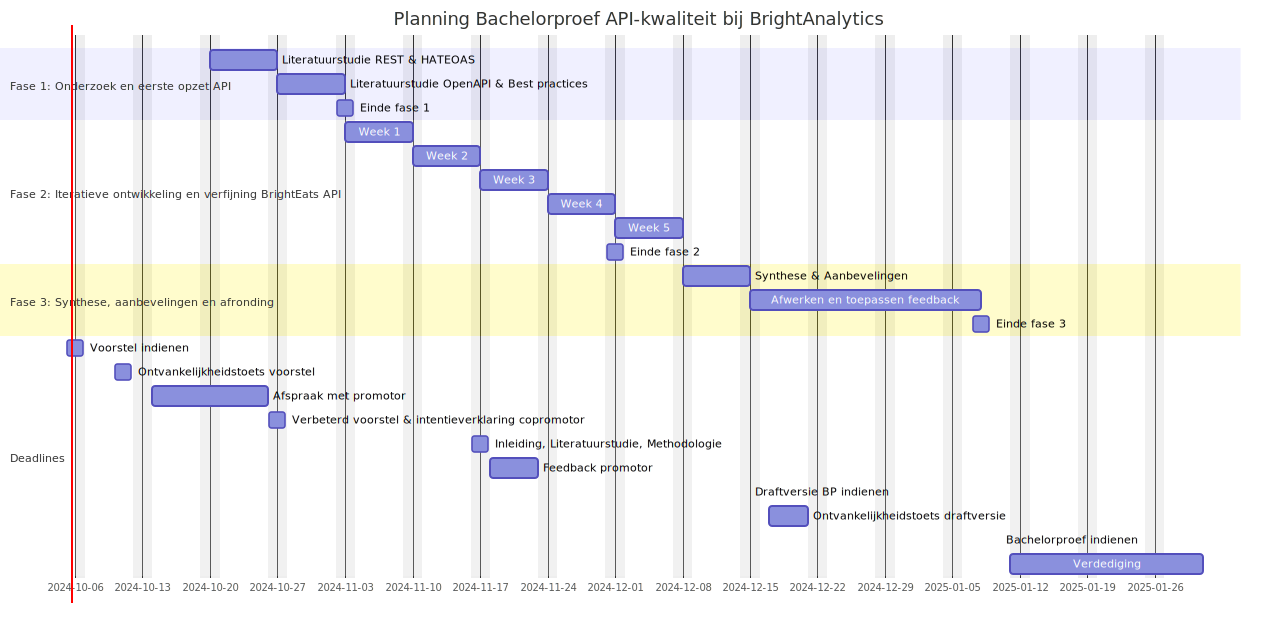
\includegraphics[width=\textwidth, keepaspectratio]{gantt-chart/gantt-chart.png}
  \caption{Gantt chart van de planning van de bachelorproef}
  \label{fig:gantt-chart}
\end{figure}
